\documentclass[a4paper]{article}

\usepackage[T1]{fontenc}
\usepackage[latin1]{inputenc}
\usepackage{ngerman}
\usepackage{listings}
\usepackage{graphicx}
\renewcommand{\figurename}{Figure}
\renewcommand{\tablename}{Table}
\usepackage{eso-pic}
\usepackage{pstricks}

\begin{document}

\begin{center}
\textbf{\LARGE{An Introduction into the\newline\newline Dresden OCL2 Toolkit for Eclipse\newline\newline}}
by Ronny Brandt and Claas Wilke
\end{center}

  These tutorial describes the work with the \textit{Dresden OCL2 Toolkit for Eclipse}. This version of the Toolkit is based on the new infrastructure called the ``pivot model"'. The pivot model was developed by Matthias Br�uer and is described in his ``Gro�er Beleg"' \cite{GBBraeuer}. Further information about the toolkit is available at the website of the Dresden OCL2 Toolkit \cite{ToolkitHP}.

	The tutorial starts with the installation of the needed \textit{Eclipse} plugins. Then it is described how to load a domain specific model and a model instance. Afterwords the importation and interpretation of OCL expressions will be explained.

  The procedure described in this tutorial is realized and tested with \textit{Eclipse 3.3.2} \cite{Ecl}. The tutorial should also run with \textit{Eclipse 3.4}. If method or menu names have been changed in \textit{Eclipse 3.4} this will be noted in the tutorial. Besides \textit{Eclipse} you also need to install the required plugins of the \textit{Eclipse Modeling Framework (EMF)}. During this tutorial the \textit{EMF} plugins of version 2.3.2 were used.
 
  To install the \textit{EMF} plugins you have to download them from the \textit{EMF} website \cite{EMF} and to extract them into the ``plugins"' directory of \textit{Eclipse}. Afterwords you can start the \textit{Eclipse SDK}. Alternatively you can install the plugins by using the \textit{Eclipse Update Manager} after starting the \textit{Eclipse SDK}.


	
	\section{How to install the Dresden OCL2 Toolkit for Eclipse}
	
	To use the \textit{Dresden OCL2 Toolkit for Eclipse} you need to install them as \textit{Eclipse} plugins, or to import them into your \textit{Eclipse workspace}. Both possibilities are explained in the following.
	
	
	\subsection{Installing the Eclipse plugins}
	
	To install the \textit{OCL2 Toolkit} as \textit{Eclipse} plugins, you need to have the jar archives of the toolkit. The jar archives are available at \cite{ToolkitSourceforge}. You need to copy the jar archives into the ``plugins"' directory of your \textit{Eclipse SDK} distribution. Then you can start the \textit{Eclipse SDK} and you can work with the Toolkit.
	
	
	\subsection{Importing the Toolkit into an Eclipse Workspace}

	Alternatively you can import the \textit{OCL2 Toolkit} as plugin projects into an \textit{Eclipse} workspace. There are two different options to do that.

On the one hand you can import the plugins from your file system, if you already have downloaded them (e.g. from \cite{ToolkitSourceforge} as a source code distribution). One the other hand you can import the plugins directly from the \textit{SVN} (\textit{Subversion}) directory of the \textit{Dresden OCL2 Toolkit}. Both possibilities are described below.

	
	\subsubsection{Import the plugins from the local file system}
	
	Let's say you have the plugins located in a directory \lstinline|XYZ| of your file system. To import them into your \textit{Eclipse} workspace you can use the \textit{Eclipse import wizard}. Open the wizard via the menu ``File > Import...`` and select  ``General > Existing Projects into Workspace"' (see figure \ref{pic:Import-EPiW}). In the following window you select the directory \lstinline|XYZ| as root. Then you select the plugins you want to import (if not selected automatically) and activate the check box ``Copy projects into workspace"' (see figure \ref{pic:ImportProjects}). After pressing the button ``Finish"' the plugins will be imported as projects into your workspace.
	
	\begin{figure}[!htbp]
		\centering
		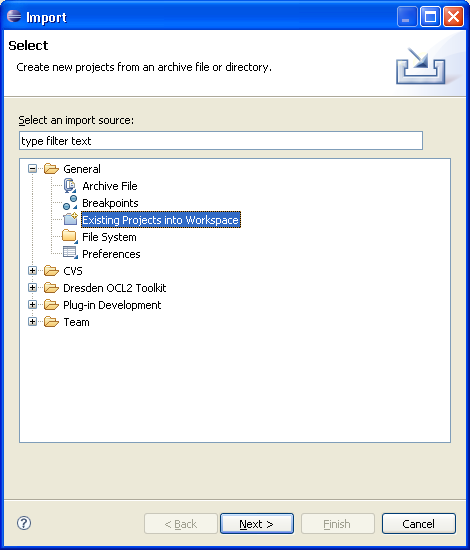
\includegraphics[width=0.8\linewidth]{figures/Import-EPiW}
		\caption{Plugin import from local file system (1).}
		\label{pic:Import-EPiW}
	\end{figure}
	
	\begin{figure}[!htbp]
		\centering
		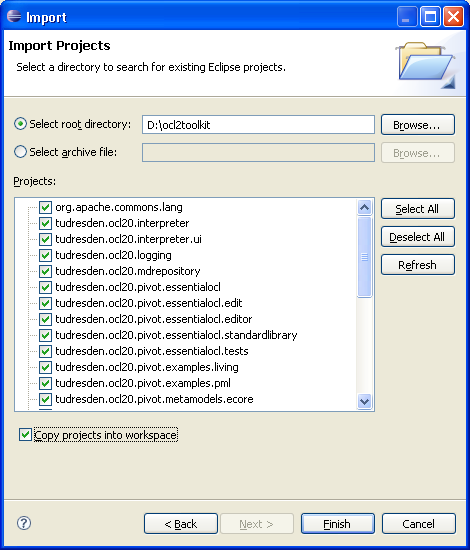
\includegraphics[width=0.8\linewidth]{figures/ImportProjects}
		\caption{Plugin import from local file system (2).}
		\label{pic:ImportProjects}
	\end{figure}
	
	
	\subsubsection{Import the plugin projects from SVN}
	
	To import the plugins directly from the \textit{SVN} repository, you need to install an additionally \textit{Eclipse} plugin to connect with the \textit{SVN}. The needed plugin is called \textit{Subclipse} (\cite{SVN}). The installation of \textit{Subclipse} is explained on the \textit{Supclipse} website \cite{SVNInstall}.
	
		\textbf{Attention: At the moment the \textit{Subclipse} plugin does not work with \textit{Eclipse 3.4}}. To access the \textit{SVN} Repository with \textit{Eclipse 3.4} use another \textit{SVN} plugin for \textit{Eclipse} or use an external tool to access the \textit{SVN} respository.
	
  After installing \textit{Subclipse} a new \textit{Eclispe perspective} for access to \textit{SVN} should exist. The perspective can be opened via the menu ``Window > Open Perpective > Other... > SVN Repository Exploring"'. In the view \textit{SVN Repository} you can add a new repository (see figure \ref{pic:SVN}) using the URL ``https://dresden-ocl.svn.sourceforge.net/svnroot/dresden-ocl/"'. After pressing the button ``Finish"' the SVN repository root should the visible in the \textit{repository view}.
	
	To checkout the plugins, you now select them in the repository directory ``trunk/ocl20forEclipse/eclipse"' and use the ``Checkout..."' function in the context menu (see figure \ref{pic:Checkout}). The given settings could be used and after a click on the ``Finish"' button the plugins should be imported.
	
	\begin{figure}[!htbp]
		\centering
		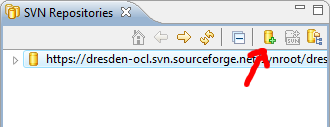
\includegraphics[width=0.5\linewidth]{figures/SVN}
		\caption{Adding an SVN repository.}
		\label{pic:SVN}
	\end{figure}
	
	\begin{figure}[!htbp]
		\centering
		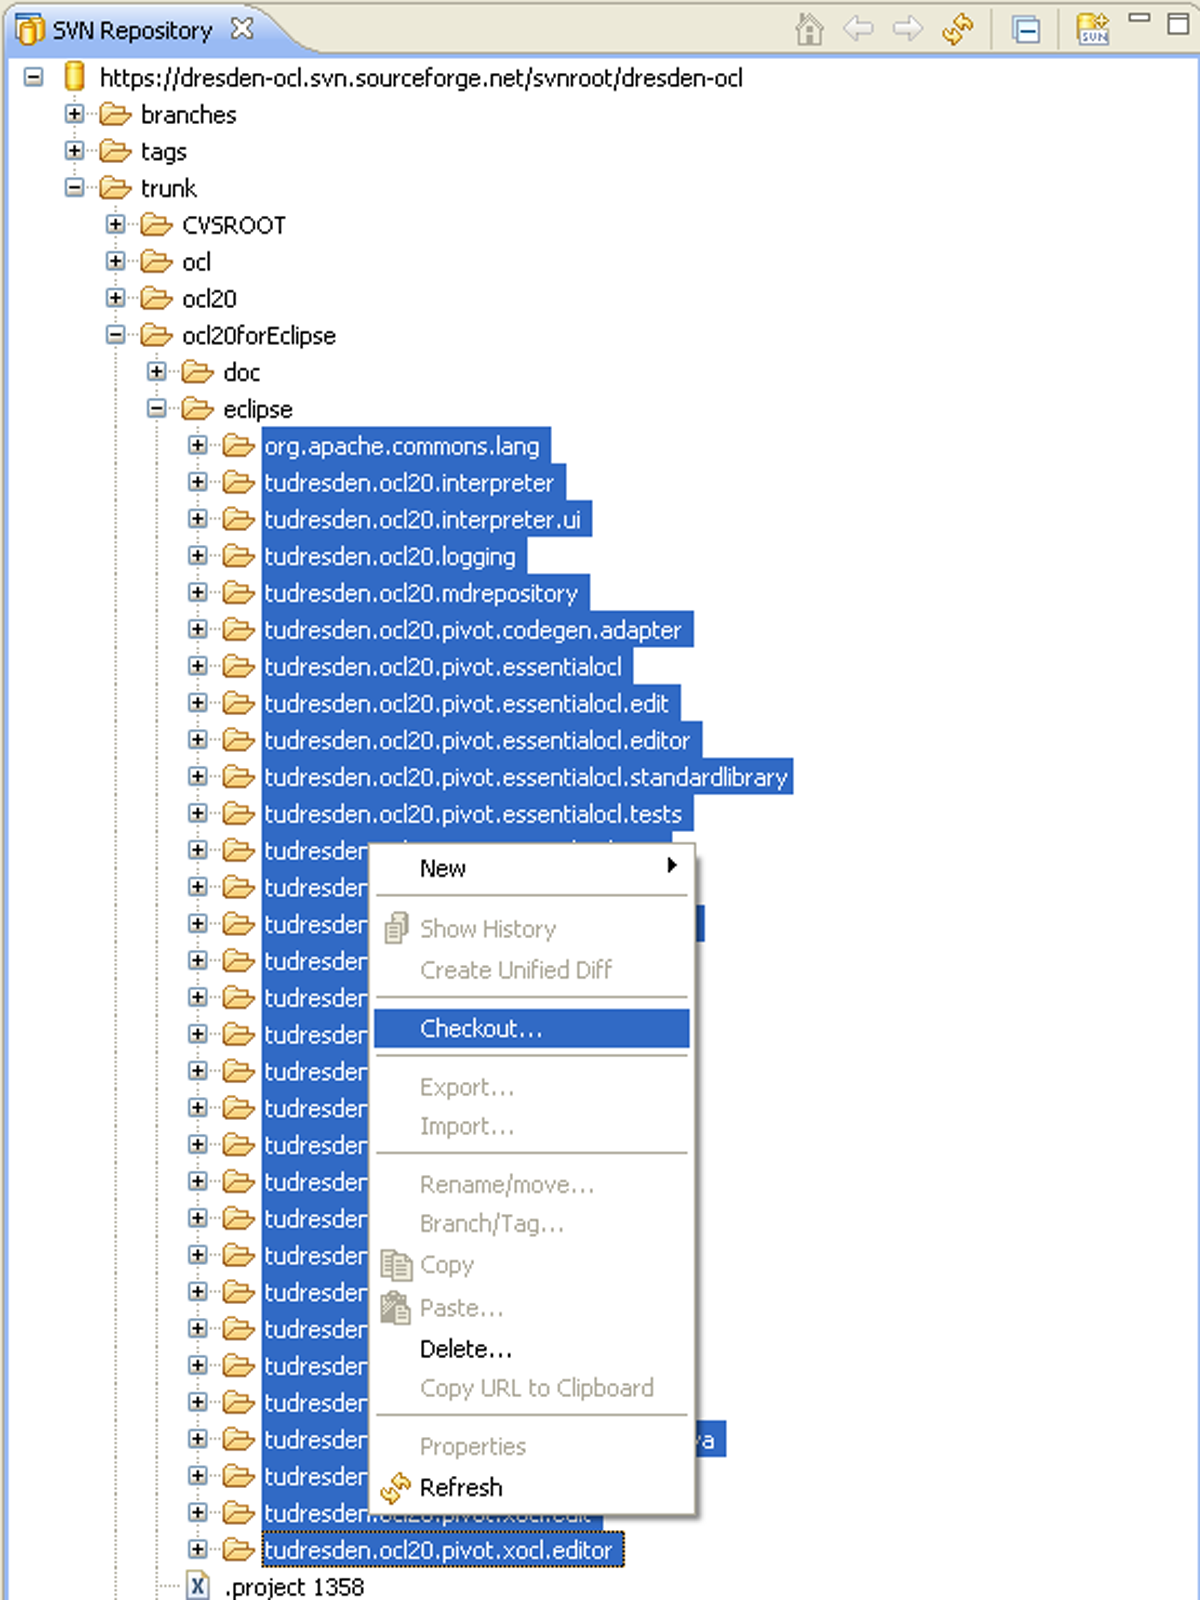
\includegraphics[width=1.0\linewidth]{figures/Checkout}
		\caption{Checkout of the Dresden OCL2 Toolkit plugin projects.}
		\label{pic:Checkout}
	\end{figure}
	
	

	\section{Building the OCL2 Parser}
	
  If you decided to run the \textit{OCL2 Toolkit for Eclipse} as project plugins into your workspace, you need to build the \textit{OCL2 Parser} of the \textit{Dresden OCL2 Toolkit for Eclipse} via an \textit{Ant} build script. If you installed the Toolkit using jar archives, you can skip this chapter of the tutorial.
  
  To build the \textit{OCL2 Parser} select the file ``build.xml"' in the project ``tudresden.ocl20.pivot.ocl2parser"' and open the context menu via a right mouse click. Select the function ``Run As ... > Ant Build"' (see figure \ref{pic:Build}).

	\begin{figure}[!htbp]
		\centering
		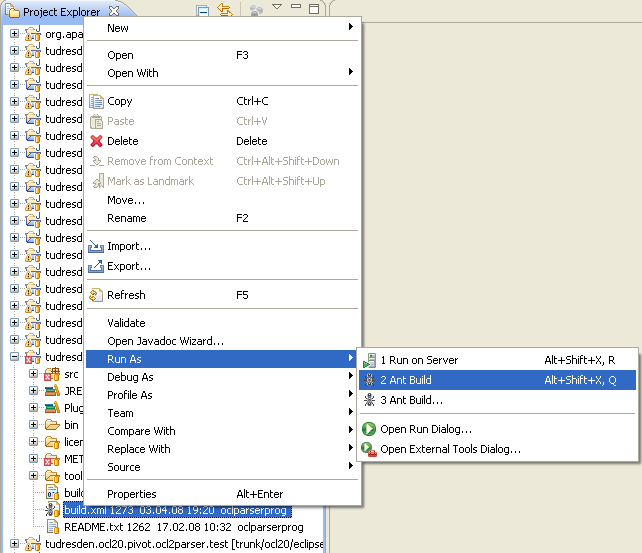
\includegraphics[width=1.0\linewidth]{figures/Build}
		\caption{Executing the OCL2 parser build script.}
		\label{pic:Build}
	\end{figure}
	
	If an error like ``Problem: failed to create task or type eclipse.refresh\-Local"' occurs, you need to change the configuration of the \textit{Ant} script. Open the function ``Properties"' in the context menu of the ``build.xml``. A new window should open. Select the topic ``Run/Debug settings"' and then the configuration for ``tudresden.ocl20.pivot.oclparser build.xml"'. Click on the button ``Edit"'. In the new window select in the sub menu ``JRE"' the check box ``Run in the same JRE as the workspace"' and click on the button ``OK"' (see figure \ref{pic:AntConfig}). Afterwords the \textit{Ant} script should be executable without errors.
	
	\begin{figure}[!htbp]
		\centering
		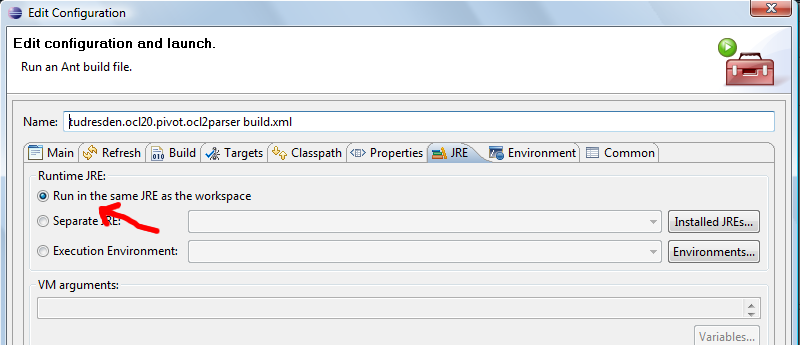
\includegraphics[width=1.0\linewidth]{figures/AntConfig}
		\caption{Settings of the JRE for the Ant build script.}
		\label{pic:AntConfig}
	\end{figure}
	
	After executing the build script successfully you need to update the projects in your workspace. Update the project ``tudresden.ocl20.pivot.oclparser"' via context menu (``Refresh"', see figure \ref{pic:Refresh}).

	\begin{figure}[!htbp]
		\centering
		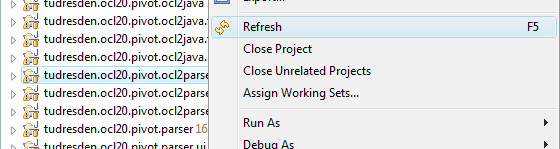
\includegraphics[width=0.5\linewidth]{figures/Refresh}
		\caption{Refreshing the project ``tudresden.ocl20.pivot.oclparser"'.}
		\label{pic:Refresh}
	\end{figure}
	
	Additionally you need to recompile all depending projects. Select the function ``Project > Clean... > Clean all projects"' in the \textit{Eclipse} menu to clean all projects. All the projects should not contain any errors anymore and should be executable.


	
	\section{Using the Dresden OCL2 Toolkit for Eclipse}

	If you installed the \textit{OCL2 Toolkit for Eclipse} using jar archives, you can execute the Toolkit by starting your \textit{Eclipse SDK}. If you imported the Toolkit as plugin projects into an \textit{Eclipse} workspace, you have to start a new \textit{Eclipse SDK} instance. You can start a new instance via the menu ``Run > Run As > Eclipse Application"'. If the menu ``Eclipse Application"' is not available or disabled you need to select one of the plugins of the toolkit first. Eventually you also have to install the \textit{Eclipse Plugin Development Environment} first. After starting the new \textit{Eclipse} instance you can use the \textit{Dresden OCL2 Toolkit for Eclipse} as described below.
	
	
	\subsection{Loading a domain specific model}
	
	After starting the \textit{Eclipse} instance you have to load a model into the toolkit. You can load a model by using the \textit{import wizard} (File~>~Import...). Select the wizard ``Dresden OCL2 Toolkit > Domain-Specific~Model"'. In a new opened window you have to select a model file and a meta model for the model (see figure \ref{pic:LoadModel}). During this tutorial the \textit{PML} Model is used which you can find in the project ``tudresden.ocl20.pivot.examples.pml"' in the file ``model/pml.ecore"'. Other examples delivered with the \textit{Dresden OCL2 Toolkit for Eclipse} are listed at the end of this tutorial.
	
	If the plugins of the \textit{Dresden OCL2 Toolkit for Eclipse} were installed as jar archives, the \textit{PML} plugin has to be imported into the \textit{Workspace} first. Create a new projekt into your \textit{Workspace} and select the \textit{import wizard} "`General -> Archive File"'; in the following windo select the "`plugins"' directory into your \textit{Eclipse} root folder, select the archive "`tudresden.ocl20.pivot.examples.living\_1.0.0.jar"' and click the "`Finish"' button.

	
	\begin{figure}[!htbp]
		\centering
		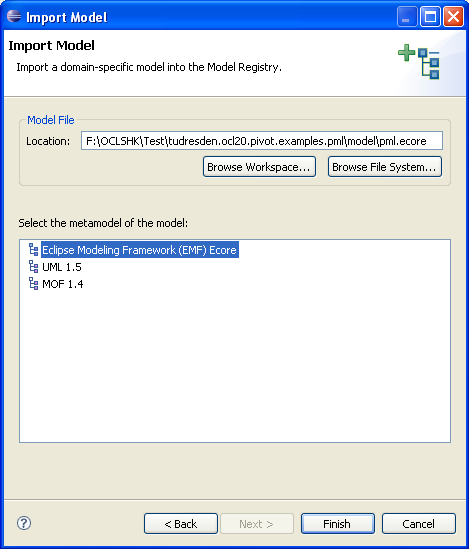
\includegraphics[width=0.8\linewidth]{figures/LoadModel}
		\caption{Loading a domain specific model.}
		\label{pic:LoadModel}
	\end{figure}
	
	Figure \ref{pic:MoBrOE} shows the loaded \textit{PML} model, which uses \textit{Ecore} as its meta model. Via the menu button (the little triangle in the right top corner) you can switch between different models in the model browser (see figure \ref{pic:SwitchModel}).
	
	\begin{figure}[!htbp]
		\centering
		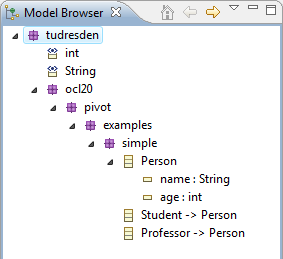
\includegraphics[width=0.5\linewidth]{figures/MoBrOE}
		\caption{The loaded PML model in the model browser.}
		\label{pic:MoBrOE}
	\end{figure}

	\begin{figure}[!htbp]
		\centering
		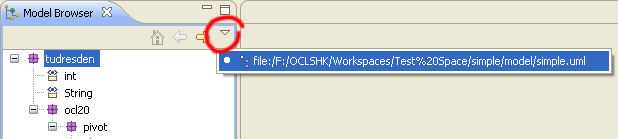
\includegraphics[width=0.8\linewidth]{figures/SwitchModel}
		\caption{You can switch between different models using the little triangle.}
		\label{pic:SwitchModel}
	\end{figure}

	
	\subsection{Loading a model instance}
	
	After loading the model, you can load a \textit{model instance} using another \textit{import wizard}. Use the wizard ``Dresden OCL2 Toolkit > Model Instance"'. You have to select a model instance (in this tutorial we used the file ``model instance/Testmodell.pml"' of the project ``tudresden.ocl20.pivot.examples.pml"') and the domain specific model loaded before (see figure \ref{pic:LoadInstance}).

	\begin{figure}[!htbp]
		\centering
		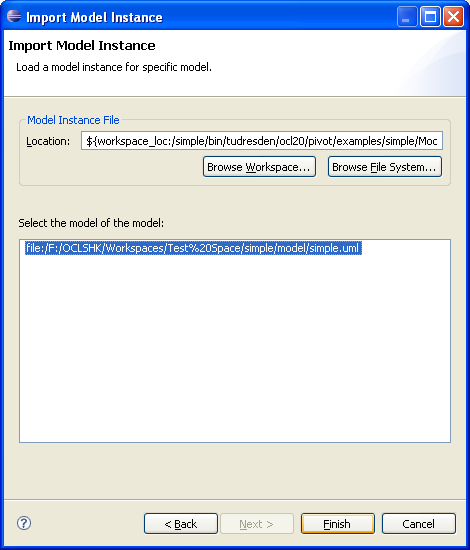
\includegraphics[width=0.8\linewidth]{figures/LoadInstance}
		\caption{Loading a \textit{PML} model instance.}
		\label{pic:LoadInstance}
	\end{figure}
	
	Figure \ref{pic:MoInBr} shows the loaded model instance of the \textit{PML} model. Like in the model browser you can switch between different model instances (after loading a model instance you could have to select the model instance first, before it appears in the model instance browser). Note that the model instance browser only shows the model instances of the model actually selected in the model browser. By switching the domain specific model, you also switch the pool of model instances available in the model instance browser.
	
	\begin{figure}[!htbp]
		\centering
		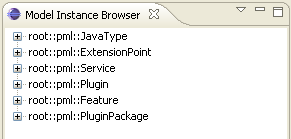
\includegraphics[width=0.5\linewidth]{figures/MoInBr}
		\caption{A loaded \textit{PML} model instance in the Model Instance Browser.}
		\label{pic:MoInBr}
	\end{figure}

	
	\subsection{Loading OCL expressions}
	\indent
	
	Before you can interprete OCL constraints you have to load them like the domain specific model and the model instance before. Use the import wizard ``Dresden OCL2 Toolkit > OCL Expressions"' and select an OCL file (in this tutorial we used the OCL file ``espressions/testpml.ocl"' of the project ``tudresden.ocl20.pivot.examples.pml"', see figure \ref{pic:LoadExpressions}).

	\begin{figure}[!htbp]
		\centering
		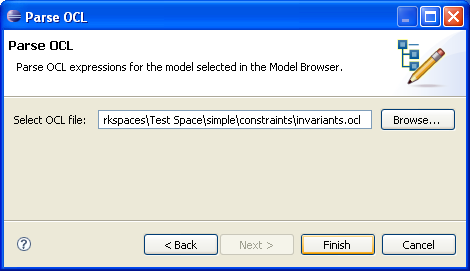
\includegraphics[width=0.8\linewidth]{figures/LoadExpressions}
		\caption{The import of OCL expressions of a model loaded before.}
		\label{pic:LoadExpressions}
	\end{figure}
	
	The expressions of the selected OCL file will be loaded into the actually selected model instance. Figure \ref{pic:MoBrME} shows the  ``Model~Browser"' containing the \textit{PML} model and the parsed expressions.
	
	\begin{figure}[!htbp]
		\centering
		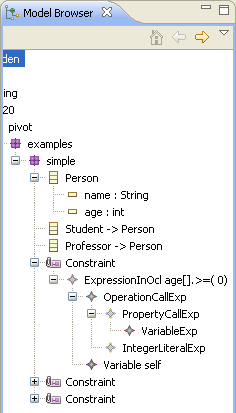
\includegraphics[width=0.5\linewidth]{figures/MoBrME}
		\caption{Parsed expressions of the \textit{PML} model in the Model Browser.}
		\label{pic:MoBrME}
	\end{figure}
	
	
	\subsection{Interpretation of constraints}
	\indent
	
	The interpretation of constraints is possible via the \textit{Interpreter View}. Eventually you have to open the \textit{View} via the menu option "`Window -> Show View -> Other..."' and select "`TU Dresden OCL2 Toolkit -> Interpreter"'.
	
	 The \textit{Interpeter View} provides a context menu containing all needed functionality. The context menu is shown in figure \ref{pic:IntViewMen} (You can open the context menu via the little triangle in the right top corner of the \textit{Interpreter View}).
	
	\begin{figure}[!htbp]
		\centering
		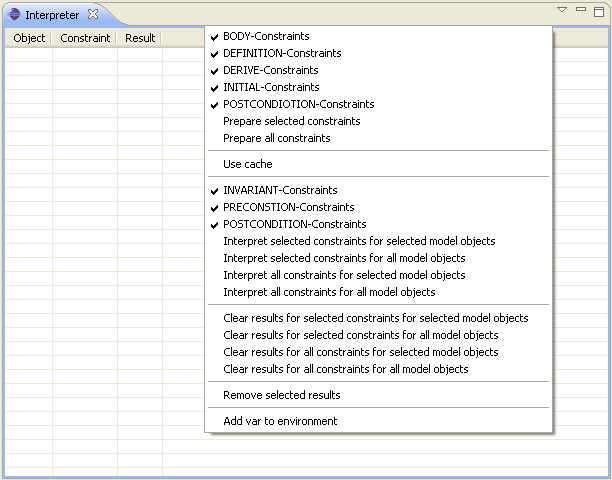
\includegraphics[width=1\linewidth]{figures/IntViewMen}
		\caption{The context menu of the \textit{Interpreter View}.}
		\label{pic:IntViewMen}
	\end{figure}
	
	For the interpretation of constraints you can use the functions ``Interpret~..."' in the context menu. First you can select constraints you want to interpret in the \textit{Model Browser} and the model objects for which the constraints should be interpreted in the \textit{Model InstanceBrowser}. The M\textit{odel Instance Browser} shows only the model objects, for which you can interpret the constraints selected before.
	
	In the \textit{interpreter menu} you can select the types you want to interpret (invariants, pre and post conditions). After interpretation the table in the \textit{Interpreter View} shows all results. These are filtered by the selection of constraints and model objects. Figure \ref{pic:IntView} shows a table with some results. If the column ``Result"' does not contain enough space for a result, you can open a result via a double mouse click in a new window.
	
	\begin{figure}[!htbp]
		\centering
		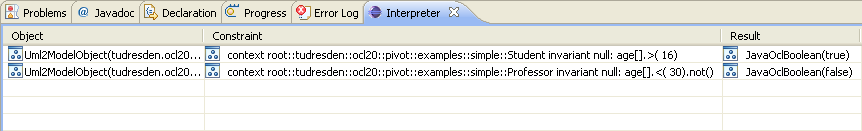
\includegraphics[width=1\linewidth]{figures/IntView}
		\caption{Some results in the \textit{Interpreter View}.}
		\label{pic:IntView}
	\end{figure}

	
	\subsection{Additional functionality of the interpreter}
	
	Before interpretation you can prepare some or all constraints like described in \cite[Abschnitt Environment]{DABrandt} (``Prepare~..."').
	
	You can add variables to the \lstinline|environment| via ``Add~var~to~environment"'. This functionality can be used for parameters and results of operations or the name of parameters. Figure \ref{pic:AVTEnv} shows a window to add variables to the environment. After entering a variable name (e.g. ``result"' or the name of a parameter) a primitive type object (e.g. Integer) can be created or the result of an already interpreted constraint can be used.
	
	\begin{figure}[!htbp]
		\centering
		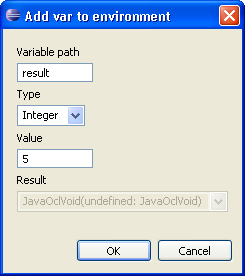
\includegraphics[width=0.4\linewidth]{figures/AVTEnv}
		\caption{Window to add a variable to the environment.}
		\label{pic:AVTEnv}
	\end{figure}
	
	Using the ``Clear~..."' functionality, results can be removed from the interpreter view. You can remove all results or select results which you want to remove before (``Remove~Selected~Results"').
	
  Using the check box ``Use~cache"', you can activate the caching mechanism described in \cite{DABrandt} to improve the performance of the interpreter.
  
  
  \section{Conclusion}
  
  This tutorial described how to use the \textit{Dresden OCL2 Toolkit for Eclipse}. It explained how to install or import and start the Toolkit's plugins. Afterwards the usage of the interpreter of the \textit{Dresden OCL2 Toolkit for Eclipse} was shown.
  	
  This tutorial explained the \textit{Dresden OCL2 Toolkit for Eclipse} using the PML example. Table \ref{tab:examples} shows all examples proviced whith the \textit{Dresden OCL2 Toolkit for Eclipse}.
	
  \begin{table}
    \begin{tabular}[h]{|r|l|}
      \hline
      \textbf{PML example} & \\
      Plugin & tudresden.ocl20.pivot.examples.pml\\
      Meta model & Ecore\\
      Model & model/pml.ecore\\
      OCL expressions & expressions/testpml.ocl\\
      Model instance & model instance/Testmodell.pml\\
      \hline
      \hline
      \textbf{Living example} & \\
      Plugin & tudresden.ocl20.pivot.examples.living\\
      Meta modell & UML 1.5 or UML 2.0\\
      Model & model/UmlExample.xmi\\
      OCL expressions & expressions/living.ocl\\
      Model instance & src/tudresden.ocl20.pivot.examples.living/ModelProviderClass.java\\
      \hline
    \end{tabular}
    \caption{Examples provided with the \textit{Dresden OCL2 Toolkit for Eclipse}.}
    \label{tab:examples}
  \end{table}

	As mentioned before, more information about the \textit{Dresden OCL2 Toolkit} is available at the website of \textit{Dresden OCL2 Toolkit} \cite{ToolkitHP}.

	\newpage
	\bibliographystyle{alphadin}
	\bibliography{tutorial_eng}

\end{document}
